\documentclass{article}
\usepackage[UTF8]{ctex}
\usepackage{graphicx}
\usepackage{caption}
\usepackage{bookman}
\usepackage{wrapfig}
\usepackage{geometry}
\usepackage{listings}
\usepackage{enumitem}
\usepackage{xcolor}
\geometry{
	a4paper,
	total={170mm,257mm},
	left=20mm,
	top=20mm,
}

\definecolor{codegreen}{rgb}{0,0.6,0}
\definecolor{codegray}{rgb}{0.5,0.5,0.5}
\definecolor{codepurple}{rgb}{0.58,0,0.82}
\definecolor{backcolour}{rgb}{0.95,0.95,0.92}

\lstdefinestyle{mystyle}{
	backgroundcolor=\color{backcolour},   
	commentstyle=\color{codegreen},
	keywordstyle=\color{magenta},
	numberstyle=\tiny\color{codegray},
	stringstyle=\color{codepurple},
	basicstyle=\ttfamily\footnotesize,
	breakatwhitespace=false,         
	breaklines=true,                 
	captionpos=b,                    
	keepspaces=true,                 
	numbers=left,                    
	numbersep=5pt,                  
	showspaces=false,                
	showstringspaces=false,
	showtabs=false,                  
	tabsize=2
}
\lstset{style=mystyle}

\graphicspath{ {./texPic/} }
%Information to be included in the title page:
\title{go实现缓存服务}
\author{潘重宇}
\date{2022/5/19}

\begin{document}
	\maketitle
	\newpage
	\paragraph{缓存服务概述}
	随着互联网的飞速发展,各行各业对互联网服务的要求也越来越高,服务架构的响应速度、数据容量一直是研究的重点。缓存服务就是为服务提速的一个方案。它需要被设置在其他服务的前端,客户端首先访问缓存查询自己的数据,仅当客户端需要的数据不存在于缓存中时,才会去访问实际的服务。从实际的服务中获取到的数据会被放在缓存中,以备下次使用。
	\paragraph{缓存与存储的关系}
	存储是非易失的,被存储的内容通常会被期望永久保存。存储对性能也有要求,比如要求系统的吞吐量达到每秒多少字节等。但在单个请求的响应时间上,存储一般不会有很高的要求。
	\\
	缓存被用来提升访问资源的速度。在设计之初,缓存就允许自己的数据出现丢失的情况,甚至有用生存时间、启发式算法来决定缓存内容的写入与回收。缓存的目的就是要快速存取。
	\section{基于HTTP的内存缓存服务}
	\paragraph{}
	使用Go语言写基于HTTP的缓存服务非常方便,我们只需要一个map来保存键值对,写一个handler来处理请求,调用http.ListenAndServe启动服务。Go的HTTP服务框架解决了底层的协议和并发问题。我们会利用HTTP/REST协议的GET/PUT/DEL方法实现缓存的Get/Set/Del操作。
	\subsection{响应流程}
	\paragraph{}
	我们以Get方法为例展示一下流程。如下图所示:
	\begin{figure}[h]
		\caption{in memory缓存的Get流程(http)}
		\centering
		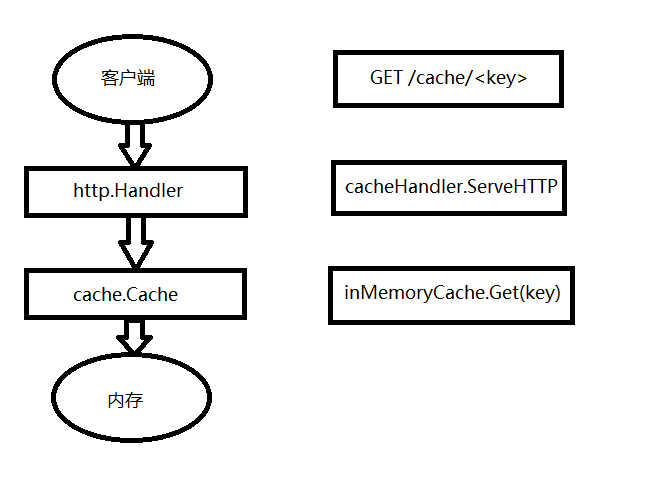
\includegraphics[width=8cm, height=6cm]{httpGet.png}
	\end{figure}
	\paragraph{}
	客户端使用HTTP的GET请求提供了key,服务端http.Handler的具体实现cacheHandler实现的SereHTTP方法负责解析客户端传来的HTTP请求,并调用cache.Cache接口的Get方法。inMemoryCache结构体的Get方法会将内存里的map(Go语言里的一种键值对数据结构)中查询key对应的value并返回。cacheHandler会将value写入HTTP的响应正文并返回200 OK。如果cache.Cache.Get返回错误,cacheHandler会返回500 Internal Server Error。如果value长度为0则返回404 Not Found。
	\subsection{cache包的实现}
	\paragraph{}
	我们希望在cache包里实现服务的缓存功能而不涉及http服务的相关内容。首先我们声明一个Cache接口:
	\begin{lstlisting}[language=Go]
		type Cache interface {
			Set(string, []byte) error
			Get(string) ([]byte, error)
			Del(string) error
			GetStat() Stat
		}
	\end{lstlisting}
	\paragraph{}
	在这个接口里,我们声明了增删查等方法。任何结构体只要实现了这些方法,我们就认为该结构体实现了Cache接口。Set用于设置键值对,它接受一个string类型的key和[]byte类型的value,返回类型为error,用于反馈操作是否成功。GetStat用于返回当前缓存的状态,类型Stat为用户定义类型的结构体。
	\begin{lstlisting}[language=Go]
		type Stat struct {
			Count     int64
			KeySize   int64
			ValueSize int64
		}
		
		func (s *Stat) add(k string, v []byte) {
			s.Count += 1
			s.KeySize += int64(len(k))
			s.ValueSize += int64(len(v))
		}
		
		func (s *Stat) del(k string, v []byte) {
			...
		}
	\end{lstlisting}
	\paragraph{}
	Cache接口可以有多种实现,在这儿我们选择实现内存内缓存inMemoryCache。它需要实现Cache里的所有方法,代码如下所示:
	\begin{lstlisting}[language=Go]
		func New(typ string) Cache {
			var c Cache
			if typ == "inmemory" {
				c = newInmemoryCache()
			}
			if c == nil {
				panic("Unknown cachetype" + typ)
			}
			log.Println(typ, "ready to server")
			return c
		}
	
		func newInmemoryCache() *inMemoryCache {
			return &inMemoryCache{make(map[string][]byte), sync.RWMutex{}, Stat{}}
		}
		
		type inMemoryCache struct {
			c     map[string][]byte
			mutex sync.RWMutex
			Stat
		}
		
		func (c *inMemoryCache) Set(k string, v []byte) error {
			c.mutex.Lock()
			defer c.mutex.Unlock()
			tmp, exist := c.c[k]
			if exist {
				c.del(k, tmp)
			}
			c.c[k] = v
			c.add(k, v)
			return nil
		}
		
		func (c *inMemoryCache) Get(k string) ([]byte, error) {
			c.mutex.RLock()
			defer c.mutex.RUnlock()
			return c.c[k], nil
		}
		
		func (c *inMemoryCache) Del(k string) error {
			...
		}
		
		func (c *inMemoryCache) GetStat() Stat {
			return c.Stat
		}
	\end{lstlisting}
	\paragraph{}
	inMemoryCache结构体包含一个类型为map的成员c,用于存储键值对;一个锁mutex用于对c提供并发读写保护;一个Stat用于记录缓存状态。Stat结构提的方法可以直接被inMemoryCache调用。
	\subsection{HTTP包的实现}
	HTTP包用来实现我们的HTTP服务功能,Go的net/http包提供了很多便利的接口于方法。服务的Server结构体代码如下:
	\begin{lstlisting}[language=Go]
		type Server struct {
			cache.Cache
		}
		
		func (s *Server) Listen() {
			http.Handle("/cache/", s.cacheHandler())
			http.Handle("/status", s.statusHandler())
			http.ListenAndServe(":12345", nil)
		}
		
		func New(c cache.Cache) *Server {
			return &Server{c}
		}
	\end{lstlisting}
	\paragraph{}
	http.Handle方法用于处理对应url路径的http请求,它接收一段string和http.Handler接口。我们需要用cacheHandler()返回http.Handler接口。具体来说是需要实现Handler接口里的ServeHTTP方法。
	\begin{lstlisting}[language=Go]
		type cacheHandler struct {
			*Server
		}
		
		func (h *cacheHandler) ServeHTTP(w http.ResponseWriter, r *http.Request) {
			key := strings.Split(r.URL.EscapedPath(), "/")[2]
			if len(key) == 0 {
				w.WriteHeader(http.StatusBadRequest)
				return
			}
			m := r.Method
			if m == http.MethodPut {
				b, _ := ioutil.ReadAll(r.Body)
				if len(b) != 0 {
					e := h.Set(key, b)
					if e != nil {
						log.Println(e)
						w.WriteHeader(http.StatusInternalServerError)
					}
				}
				return
			}
			...
			w.WriteHeader(http.StatusMethodNotAllowed)
		}
		
		func (s *Server) cacheHandler() http.Handler {
			return &cacheHandler{s}
		}
	\end{lstlisting}
	\subsection{main包实现}
	\paragraph{}
	最后是main包的内容:
	\begin{lstlisting}[language=Go]
		func main() {
			c := cache.New("inmemory")
			HTTP.New(c).Listen()
		}
	\end{lstlisting}

	\section{基于TCP的内存缓存服务}
	\paragraph{}
	抛弃Golang自身的HTTP框架意味着我们需要处理TCP连接和并发的请求,自己定义和解析tcp传输的网络字节流。大致流程如下所示:
	\begin{figure}[h]
		\caption{in memory缓存的Get流程(TCP)}
		\centering
		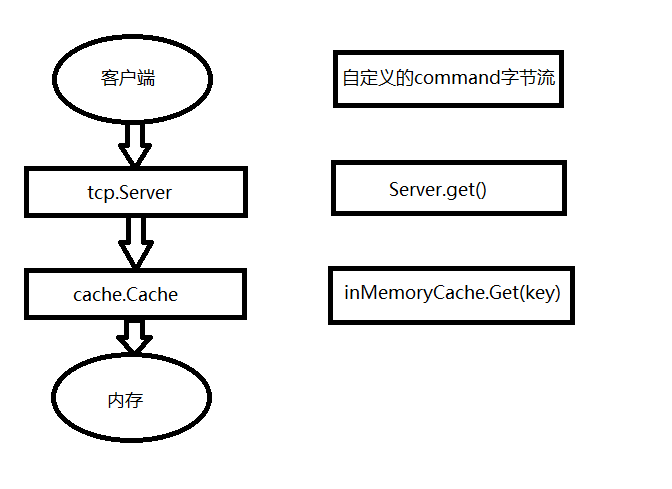
\includegraphics[width=8cm, height=6cm]{tcpGet.png}
	\end{figure}
	\paragraph{}
	幸运的是我们只需要解决这些问题,并且go有着便利的goroutine用于并发。流程图中的cache包已经在上一节中实现了,我们只需要实现tcp包的相关内容。
	\subsection{TCP包的实现}
	和HTTP包一样,我们需要一个Server结构体来处理TCP连接以及客户端交互。它的Listen()方法使用一个无线循环接受12346端口的客户端连接请求,并在goroutine上调用process()来处理请求:
	\begin{lstlisting}[language=Go]
		type Server struct {
			cache.Cache
		}
		
		func (s *Server) Listen() {
			l, e := net.Listen("tcp", ":12346")
			if e != nil {
				panic(e)
			}
			for {
				c, e := l.Accept()
				if e != nil {
					panic(e)
				}
				go s.process(c)
			}
		}
		
		func New(c cache.Cache) *Server {
			return &Server{c}
		}
	\end{lstlisting}
	\paragraph{}
	其中Server.process()的相关实现如下所示:
	\begin{lstlisting}[language=Go]
		func (s *Server) readKey(r *bufio.Reader) (string, error) {
			klen, e := readLen(r)
			if e != nil {
				return "", e
			}
			k := make([]byte, klen)
			_, e = io.ReadFull(r, k)
			if e != nil {
				return "", e
			}
			return string(k), nil
		}
		
		func (s *Server) readKeyAndValue(r *bufio.Reader) (string, []byte, error) {
			...
		}
		
		func readLen(r *bufio.Reader) (int, error) {
			//以空格为分隔符读取下一段字符串并转化为一个整型
			...
		}
		
		func sendResponse(value []byte, err error, conn net.Conn) error {
			if err != nil {
				errString := err.Error()
				tmp := fmt.Sprintf("-%d ", len(errString)) + errString
				_, e := conn.Write([]byte(tmp))
				return e
			}
			vlen := fmt.Sprintf("%d ", len(value))
			_, e := conn.Write(append([]byte(vlen), value...))
			return e
		}
		
		func (s *Server) get(conn net.Conn, r *bufio.Reader) error {
			k, e := s.readKey(r)
			if e != nil {
				return e
			}
			v, e := s.Get(k)
			return sendResponse(v, e, conn)
		}
		
		func (s *Server) set(conn net.Conn, r *bufio.Reader) error {
			...
		}
		
		func (s *Server) del(conn net.Conn, r *bufio.Reader) error {
			...
		}
		
		func (s *Server) process(conn net.Conn) {
			defer conn.Close()
			r := bufio.NewReader(conn)
			for {
				op, e := r.ReadByte()
				if e != nil {
					if e != io.EOF {
						log.Println("close connection due to error", e)
					}
					return
				}
				if op == 'S' {
					e = s.set(conn, r)
				} else if op == 'G' {
					e = s.get(conn, r)
				} else if op == 'D' {
					e = s.del(conn, r)
				} else {
					log.Println("close connection due to invalid operation:", op)
					return
				}
				if e != nil {
					log.Println("close connection due to error:", e)
					return
				}
			}
		}
	\end{lstlisting}
\end{document}